\documentclass[main]{subfiles}
\begin{document}

%@@@@@@@@@@@@@@@@@@@@@@@@@@@@@@
% Main Topics: projection of polyhedra, Fourier-Motzkin elimination
% Formally defining projection of a polyhedra - 02.10.2017
% author: Vanessa Leite

\section{Projection of Polyhedra}

\subsection{Elimination of one variable}
\paragraph{Definition: Let $S \subseteq \mathbb{R}^{n}$. $Proj_{x_{1}}, \dots,
x_{n-k} (S) = \{ (x_{1}, \dots, x_{n-k}) \in \mathbb{R}^{n-k} \mid \exists
x_{n-k+1}, \dots, x_{n}$ such that $(x_{1}, \dots, x_{n-k -1}, x_{n-k}, \dots,
x_{n}) \in S \}$.} See figure~\ref{fig:projection}. \\

\begin{figure}[!h]
  \label{fig:projection}
  \centering
    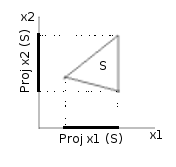
\includegraphics{imgs/projection.png}
\end{figure}

Notation: Let $P = \{x \in \mathbb{R}^n \mid Ax \leq b\} = \{x \in \mathbb{R}^n
\mid \sum_{j = 1}^{n} a_{ij}x_{j} \leq b_{i}$, $\forall i \in M \}$

For $x \in \mathbb{R}^n$, $\bar{x} =
\begin{pmatrix}
	x_1 \\
    \dots \\
    x_{n-1}
\end{pmatrix}$ (we drop the last variable).
$\bar{A} = [A_{\cdot 1} | \dots | A_{\cdot (n-1)}]$

\subsubsection{Algorithm to compute projection ($proj_{\bar{x}}(P)$)}
\paragraph{01. Rewrite the system $Ax \leq b$ in another way: by isolating one
variable and normalizing.}

$Ax \leq b = a_{i n} x_{n} \leq b_i - \sum_{j = 1}^{n-1} a_{ij}x_j \forall i
\in M$.
Then, we obtain a new representation:
$x_n \leq d_i + f_i^T \bar{x} \forall i$ such that $a_{in} > 0$,
$x_n \geq d_i + f_i^T \bar{x} \forall i $ such that $a_{in} < 0$,
$0 \leq d_k + f_k^T \bar{x} \forall k $ such that $a_{kn} = 0$.
where, $d_i = \frac{b_i}{a_{in}}$ and $f_i = -(\frac{a_{ij}}{a_{in}}) \forall j
= 1, \dots, n-1$.

\paragraph{02. Define $Q = \{\bar{x} \in \mathbb{R}^{n-1} \mid d_j + f_j^T
\bar{x} \leq d_i + f_i^T \bar{x} \forall j, i$ such that $a_{in} > 0$, $a_{jn}
<0$ and $0\leq d_k +f_k^T \bar{x} \forall k$ such that $a_{kn} = 0\}$ }


Standard form: $f_j^T \bar{x} - f_i^T x \leq d_i - d_j$


\textbf{In the worst case, the number of constraints generated by the algorithm
goes to $m^2$, considering $m$ is the original number of constraints.}

\paragraph{03. Return $Q$}


\textbf{Theorem: $Q = proj_{\bar{x}}(P)$ (we verify the number of constraints
in $Q$ match the dimension)}

\subparagraph{Proof: "$proj_{\bar{x}} (P) \subseteq Q$"}
Let $\bar{x} \in proj_{\bar{x}}(P) \rightarrow \exists x_n$ such that
$(\bar{x}, x_n) \in P$. Then $(\bar{x}, x_n)$ satiesfies the new representation
in the first step of the algorithm. Thus, $\bar{x} \in Q$.

\subparagraph{Proof: "$Q \subseteq proj_{\bar{x}}(P)$"}
Let $\bar{x} \in Q$. Let $L:= max \{d_j + f_j^T \bar{x} \mid a_{jn} < 0 \}$ 
and $U:= min \{ d_i + f_i^T \bar{x} \mid a_{in} > 0 \}$.
$L \leq U$, since $\bar{x} \in Q$. Take any $x_n \in [L, U]$. Then $(\bar{x},
x_n)$ satisfies the new representation in the first step of the algorithm.
Thus, $\bar{x} \in proj_{\bar{x}}(P)$.\\

\emph{Projection is a key algebraic operator for duality}

\subsection{The special case of dimension 1}
Take a polyhedron in dimension 1 (an interval): $P \subseteq \mathbb{R}$.
Let $a \in (\mathbb{Q}\setminus \{0\})^m$, $b \in \mathbb{Q}^m$. $P = \{ x \in
\mathbb{R} \mid ax \leq b \}$, we can rewrite $P$ as: $P = \{ x \in \mathbb{R}
\mid l \leq x \leq u \}$, $l = max \{ \frac{b_i}{a_i} \mid a_i < 0 \}$ and $u =
min \{ \frac{b_i}{a_i} \mid a_i > 0 \}$.

\paragraph{When the polyhedron is empty $(P = \emptyset)$?}
$P = \emptyset \iff l > u \iff 0 > u-l$. This conclusion can be derived from
the original representation of $P$.

\paragraph{Usin a projection}
$proj_{0}(P) = \{ 0 \leq y^T b$ $\forall y \geq 0$, $y^T a = 0 \}$ \\
Observation: $P \neq \emptyset \iff 0 \leq y^T b$ $\forall y \geq 0$ such that
$y^T a = 0$.

\subsection{Repeated projections}
Observation: $proj_{(x_1, \dots, x_{n-2})}(P) = proj_{(x_1, \dots, x_{n-2})}
proj_{(x_1, \dots, x_{n-1})}(P))$.

\textbf{Theorem: Let $P = P^{(0)} = \{ x \in \mathbb{R}^n \mid Ax \leq b \}$.
Define a submatrix $A^{(j)}$ of matrix $A$ with columns $A_{\cdot k} \forall k
\in \{1, \dots, j\}$. Also define a set $C^{(0)} = \mathbb{R}_+^m$. $C^{(i)} =
\{ y \in \mathbb{R}_+^m \mid y^T A_{\cdot k} = 0$ $\forall k = n-i+1, \dots, n
\} = \{y \in C^{(i-1)} \mid y^T A_{\cdot (n-i+1)} = 0\}$ }

Then $proj_{(x_1, \dots, x_{n-i})}(P)$ can be described by half-spaces:
$P^{(i)} = \{ \bar{x} \in \mathbb{R}^{n-i} \mid y^T A^{(n-i)}x \leq y^T b$
$\forall y \in C^{(i)} \}$.

\subparagraph{Proof: "$proj_{(x_1, \dots, x_{n-i})} \subseteq P^{(i)}$"}
Take $(x_1, \dots, x_{n-i}) \in proj_{x_1, \dots, x_{n-i}}(P).$ $\exists x \in
\mathbb{R}^j$ such that
$\begin{pmatrix}
	x_1 \\
    \dots \\
    x_{n-1} \\
    z
\end{pmatrix} \in P$.

Take any $y \in C^{(i)}$: Show $y^T A^{(n-i)} x \leq y^T b$, $y \geq 0$.
$\sum_{j=1}^{n-i} A_{\cdot j}x_j + \sum_{j = n-i + 1}^n A_{\cdot j} z_j \leq b
\rightarrow \sum_{j = 1}^{n-i} y^T A_{\cdot j} x_j +
\underbrace{\sum_{j=n-i+1}^{n} y^T A_{\cdot j} z_j}_{=0 \text{, because } y \in
C^{(i)}} \leq y^T b$.

$\iff y^T A^{(n-i)} \leq y^T b$.

\subparagraph{Proof: "$P^{(i)} \subseteq proj_{(x_1, \dots, x_{n-i})}(P)$"}

We perform induction on $i$. \\
$i = 0 \rightarrow$ trivial. \\
Suppose our theorem applies for indices up to $j-1$. Consider index $j$.\\
What we know: the $proj_{(x_1, \dots, x_{n-j})}(P) = proj_{(x_1, \dots,
x_{n-j})}(proj_{(x_1, \dots, x_{n-j+1})}(P)$.\\

Inductive argument: $proj_{(x_1, \dots, x_{n-j})}(P) = P^{(j-1)} =
\underbrace{ \{ x \mid y^T A^{(n-j+1)} x \leq y^T b \forall y \in C^{(j-1)}
\} }_{\text{infinite, but redundat}}$ = $\{x \in \mathbb{R}^{n-j+1} \mid
\underbrace{Bx \leq d}_{\text{finite constraints}} \}$.

Define:\\
$M_+ = \{i \in M \mid B_{i, n-j+1} > 0 \}$\\
$M_- = \{i \in M \mid B_{i, n-j+1} < 0 \}$\\
$M_0 = \{i \in M \mid B_{i, n-j+1} = 0 \}$\\

Then, $proj_{(x_1, \dots, x_{n-j})}(P^{(j-1)}) = Q \overbrace{=}^{\text{first
theorem}} \{ \bar{x} \in \mathbb{R}^{n-j} \mid (a) \sum_{k=1}^{n-j} B_{j,k}
\bar{x}_k \leq d_i \forall i \in M_0$, $(b) \sum_{k=1}^{n-j} (\frac{B_{r,k}}
{B_{r, n-j+1}} - \frac{B_{s,k}}{B_{s, n-j+1}}) \bar{x}_k \leq \frac{d_r}{B_{r,
n-j+1}} - \frac{d_s}{B_{s, n-j+1}}$, $\forall r \in M_+$, $s \in M_- \}$.

\textbf{Claim: Every constraint of type $(a)$, $(b)$ in $Q$ is a constraint in
$P^{(i)}$.}\\
Take a constraint of type $(a)$ in $Q$. We know $i \in M_0$ and the induction
implies $\exists y \in C^{(j-1)}$ such that $y^T A^{(n-j+1)} = B_i$. Since
$B_{i, n-j+1} = 0 \rightarrow y \in C^{(j)}$.\\

Take a constraint of type $(b)$ in $Q$. Inductive argument shows $\exists y^r
\in C^{(j-1)}$, $y^s \in C^{(j-1)}$ such that $(y^r)^T A^{n-j+1} = B_r$,
$(y^s)^T A^{n-j+1} = B_s$.

$y = \frac{1}{B_{r, n-j+1}} y^r - \frac{1}{B_{s, n-j+1}} y^s \in C^{(j)}
\rightarrow y^T A_{\cdot (n-j+1)} = 0$ and $y \geq 0$, $y \in C^{(j-1)}
\rightarrow y \in C^{(j)}$.
\end{document}
